\documentclass[pdflatex,sn-nature,iicol]{sn-jnl}
\usepackage{graphicx}
\usepackage{amsmath,amssymb}
\usepackage{booktabs}
\usepackage{array}
\usepackage{float}
\renewcommand{\topfraction}{0.95}
\renewcommand{\dbltopfraction}{0.95}
\renewcommand{\textfraction}{0.05}
\setlength{\dbltextfloatsep}{10pt plus 2pt minus 2pt}
\setlength{\dblfloatsep}{12pt plus 2pt minus 2pt}
\AtBeginDocument{\setlength{\bibsep}{0pt}\def\bibfont{\footnotesize}}
\begin{document}
\title[Evidence from wall-model tests]{When can a wall-model test support a new prediction?}
\author{\fnm{Authors:} \sur{to be decided}}
\abstract{In a statistically stationary, fully developed symmetric plane channel, a prescribed pressure gradient fixes the mean wall stress, so agreement on it checks the momentum balance, not the wall law. We review what published wall-model tests establish for a new prediction. In 136 controlled comparisons from 58 reports, only the wall treatment changes. One treatment lies closer to the reference wherever a direction is resolved in 29. In 27 the closer treatment changes between conditions, most often with the grid or the Reynolds number, or between quantities. In 55 more it changes only along one profile. Behind a backward-facing step, a graph wall model moves mean reattachment from about 4.7 to 5.2 step heights, against 6.0 in a wall-resolved simulation. Three comparisons are worked through to a discriminating next test. Whether the five-question checklist, tried on 13 retrospective cases, improves prospective decisions remains open.}
\keywords{wall model, turbulence, large-eddy simulation, generalisation, validation}
\maketitle

\section{Introduction}\label{sec:intro}
Suppose a wall-modelled large-eddy simulation (LES) must locate mean reattachment behind a step to within half a step height. In the coupled calculations of Dupuy et al.~\cite{Dupuy2023graph}, a graph wall model reduces two integrated stress errors relative to a log law. Its reattachment point is still about 0.8 step heights upstream of the wall-resolved benchmark. That point estimate gives insufficient grounds to claim the illustrative half-step accuracy.

\begin{figure*}[t]
\fbox{\parbox{\dimexpr\textwidth-2\fboxsep-2\fboxrule\relax}{\fontsize{8}{9.5}\selectfont\setlength{\parskip}{3pt}%
\textbf{Box 1 \textbar{} Search, selection and data extraction}\par
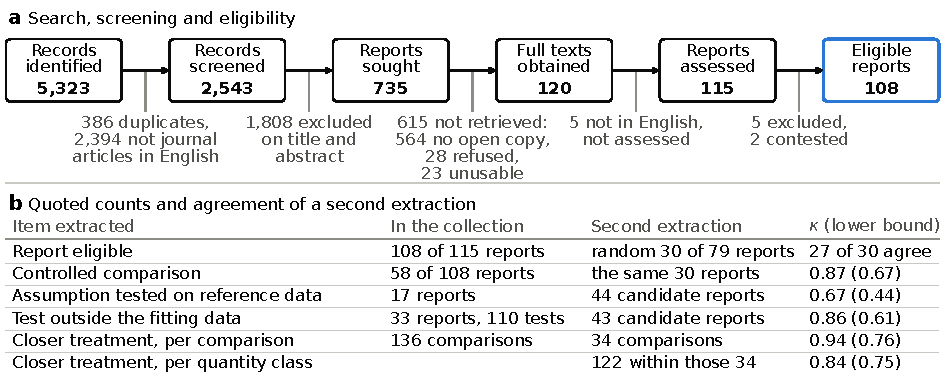
\includegraphics[width=\linewidth]{../figures/box1_flow.pdf}\par
We chose examples that distinguish competing explanations for a wall-stress error or expose ambiguities in a comparison. An OpenAlex search of journal records from 2000 to November 2026 supplied an initial collection. We also consulted earlier work on wall laws, independent studies of numerical error and papers cited by the selected studies. Figure~\ref{fig:record} compares eight studies by flow geometry. The bibliography identifies the preprints and accepted manuscript used for particular readings.

An earlier analysis grouped 82 study treatments. We re-examined the eligibility decisions for the other 33 records in the archived set, including the distinction between a wall-stress estimate and a test in a coupled solver. Inconsistent treatment of those tests and of thermal and hydrodynamic evidence prevented a reliable field-wide count. We withdrew estimates of how often tests supported transfer beyond calibration and how often conclusions changed with the measured quantity alone. A paper excluded on physical grounds may still contain a coupled validation. The repository gives the original decisions and corrections.
}}
\end{figure*}

Oberkampf and Trucano~\cite{OberkampfTrucano2002} distinguish verification of the numerical solution, validation against experiment and prediction outside tested conditions. ASME V\&V~20 assesses accuracy for a specified variable at a validation point, accounting for uncertainty in the solution and the measurements. Extrapolation calls for engineering judgement~\cite{ASMEVV20}. We apply these principles by asking what constrained the measured quantity in the published calculation and what could change it in the intended one.

Cabot and Moin~\cite{CabotMoin2000} distinguished accuracy in the core of the flow from accuracy close to the wall. Piomelli and Balaras~\cite{PiomelliBalaras2002} reviewed the range of applicability of wall-layer models. Bose and Park~\cite{BosePark2018} examined when the momentum terms neglected by equilibrium models matter. Larsson et al.~\cite{Larsson2016} showed how to refine an LES grid at a fixed physical sampling height. The community guide to wall-modelled LES~\cite{WMLESValidation} recommends choosing the measured quantity with other sources of error in mind. Behind the step, the graph predicts stress magnitude from neighbouring grid points and the first off-wall velocity sets its direction~\cite{Dupuy2023graph}. Refining the grid moves both inputs.

For learned closures, Hu and Yang~\cite{HuYang2026} identify the mismatch between training on reference data and \emph{a posteriori} performance and propose statistical tests. Vadrot et al.~\cite{Vadrot2023} compared three learned wall models with an equilibrium law in one solver across Reynolds numbers in half-channel flow. The two supervised models recovered logarithmic behaviour, one with a different slope, and the reinforcement-trained model's shift in mean velocity changed sign with Reynolds number. The imposed pressure gradient constrains the mean wall force, leaving these profile differences informative.

At high Reynolds number the cost of resolving a wall makes such decisions consequential. For a flat-plate boundary layer, Choi and Moin~\cite{ChoiMoin2012} estimated that the number of grid points grows as $Re_L^{13/7}$ for wall-resolved LES and as $Re_L$ for wall-modelled LES, where $Re_L$ uses the plate length. 

This Review first states what the forcing and the momentum balance already fix in a test, and so which outputs can test a wall law (Sec.~\ref{sec:framework}). It then examines what published comparisons establish, in eight examples and in the 136 controlled comparisons found by a documented search (Sec.~\ref{sec:evidence}, Box~1, Sec.~\ref{sec:methods}), recording which of two wall treatments lies closer to the reference in every quantity compared. Section~\ref{sec:procedure} works three comparisons through to a next test that differs from plain grid refinement.

\begin{figure*}[t]
\centering
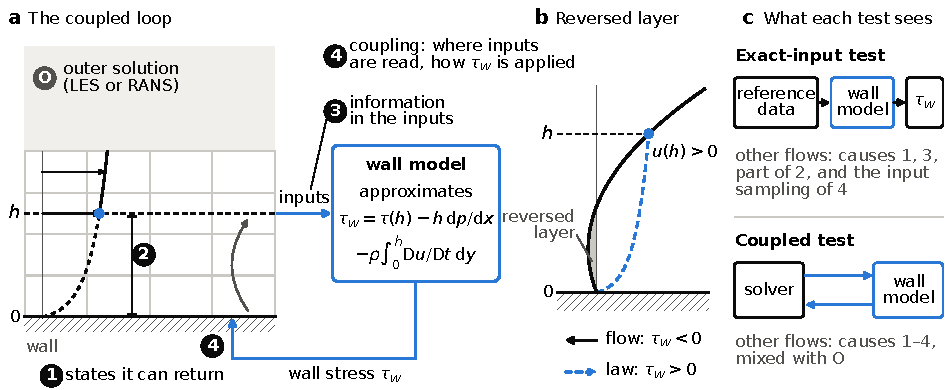
\includegraphics[width=\textwidth]{../figures/fig1_loop.pdf}
\caption{Where limitations enter a wall-modelled calculation. \textbf{a}, The model samples the flow at height $h$. The box shows the mean thin-layer balance with zero body force and mean-flow acceleration $a_x$. The returned stress uses the fluid-on-wall sign. The curved arrow shows feedback. The dashed profile is modelled. Numbers denote admissible stresses (1), momentum balance (2), inputs (3) and coupling (4). O denotes contributions outside the model. \textbf{b}, At one instant the velocity at $h$ is positive and the wall gradient is negative. An aligned law given this sample cannot return the required negative shear. Both profiles are schematic. \textbf{c}, An \emph{a priori} test prescribes the inputs and tests the wall law directly. In an \emph{a posteriori} (coupled) test its stress affects the next velocity sample.}\label{fig:loop}
\end{figure*}

\section{A physical framework for assessing evidence}\label{sec:framework}
Take a stationary, impermeable lower wall at $y=0$, with $x$ downstream and $y$ into the fluid. For incompressible flow of constant density $\rho$ and viscosity $\mu$, let $(U,V)$ and $p$ be the ensemble-mean velocities and pressure in a two-dimensional mean flow. The acceleration of that mean is $a_x=\partial_t U+U\partial_x U+V\partial_y U$. Fluctuations about it transport momentum. The signed total fluid shear is $\tau=\mu(\partial_y U+\partial_x V)-\rho\langle u'v'\rangle$, where brackets denote the same average. For filtered LES fields the turbulent flux includes both the resolved covariance and the mean subgrid momentum flux.

In the thin-layer approximation~\cite{BosePark2018}, pressure is uniform across the layer and streamwise gradients of viscous and turbulent stresses are neglected. With mean body acceleration $f_x$, the retained balance is $\rho a_x=-\partial_xp+\partial_y\tau+\rho f_x$. Integrating from the wall to the sampling height $h$ gives
\begin{equation}
\tau_w=\tau(h)-h\,\frac{\partial p}{\partial x}
+\rho\int_0^h(f_x-a_x)\,\mathrm{d}y .
\label{eq:balance}
\end{equation}
The outward fluid normal is $-\hat{\boldsymbol y}$. The streamwise traction exerted by the wall on the fluid is $-\tau(0)$, and the fluid exerts $\tau_w=\tau(0)$ on the wall. At a smooth no-slip wall, $\tau_w=\mu\,\partial_y U|_0$. Equation~\eqref{eq:balance} is an identity of the retained equation. Strong separation, curvature or spanwise variation can require additional stress transport.

In a statistically stationary, fully developed symmetric plane channel of half-height $\delta$, take time and wall-parallel plane means. For pressure driving alone ($\mathrm{d}p/\mathrm{d}x<0$, $f_x=0$), $a_x=0$ and the \emph{exact} mean momentum equation reduces to $\mathrm{d}\tau/\mathrm{d}y=\mathrm{d}p/\mathrm{d}x$. Centreline symmetry gives $\tau(\delta)=0$, hence $\tau_w=-\delta\,\mathrm{d}p/\mathrm{d}x$ and $\tau(h)=\tau_w(1-h/\delta)$. The largest fractional drop across the layer is $h/\delta$. Constant stress is accurate for $h\ll\delta$, even though the pressure contribution is finite at every $h>0$.

More generally, stress is approximately uniform when the accumulated non-shear terms stay small relative to a nonzero wall-stress scale at every height in the layer. In a developing layer, nearly equal endpoint stresses alone leave interior variation open. Attributing a small change to cancellation requires appreciable, oppositely signed pressure and acceleration contributions, measured over the same layer with the same averaging, whose sum matches $\tau_w-\tau(h)$ within the closure error of the budget.

An algebraic wall law adds an assumption about the velocity profile. Spalding's relation~\cite{Spalding1961}, for example, connects the mean velocity to distance from a smooth wall in wall units. Using an instantaneous LES velocity in such a relation introduces a further modelling assumption. Near separation, the friction velocity tends to zero and velocity or pressure-gradient measures normalised by it become singular~\cite{BosePark2018}.

The direction test in Fig.~\ref{fig:loop}b pairs the input with the reference traction at the same station and instant, using the filters specified by the law. Opposite streamwise signs exclude alignment for that sample. The means can have opposite signs even under perfect instantaneous alignment. For four equally weighted velocities $u_h=(1,1,1,-2)$, the aligned law $|u_h|u_h$ gives mean velocity $1/4$ and mean stress $-1/4$ in dimensionless units. A law evaluated on the mean velocity makes a separate, directly testable prediction.

The other questions in Fig.~\ref{fig:loop} concern the balance, the inputs and the coupling. Park and Moin~\cite{ParkMoin2014} retained unsteadiness and three-dimensional transport in their near-wall RANS equations, with turbulent stresses still requiring closure. After a change in forcing, two profiles can have the same instantaneous velocity at $h$ and different wall gradients. A law given only that velocity must give the same stress for both.

The boundary condition matters. Bae et al.~\cite{Bae2018} used a dynamic slip (Robin) condition relating filtered velocity to its wall-normal derivative, with transpiration at the solid wall. Its admissible stresses follow from that condition. An \emph{a priori} comparison tests a response for prescribed inputs. An \emph{a posteriori} comparison includes feedback, outer discretisation, subgrid closure and boundary conditions. A wall-resolved simulation supplies a numerical benchmark with its own discretisation and finite-sampling uncertainties~\cite{OberkampfTrucano2002,Oliver2014}.

\begin{table*}[t]
\caption{Forcing and informative outputs in statistically stationary flow. In the fully developed smooth ducts, $G=-\mathrm{d}p/\mathrm{d}x$ is the mean pressure drop per unit length, $\delta$ the channel half-height and $R$ the pipe radius. Drag is the downstream force of fluid on walls. On periodic hills the drive is represented by a body force with periodic pressure.}\label{tab:tests}
\footnotesize
\begin{tabular*}{\textwidth}{@{\extracolsep{\fill}}p{0.28\textwidth}p{0.30\textwidth}p{0.35\textwidth}@{}}
\toprule
Set-up & Imposed quantity or balance & Further outputs to assess \\
\midrule
Plane channel or circular pipe, prescribed $G$ & Mean drag per wetted area equals $G\delta$ in the channel and $GR/2$ in the pipe & Bulk velocity, profile shape and fluctuations \\
Channel or pipe, prescribed bulk flow rate & Bulk velocity & Required $G$ and corresponding mean drag per area, linked as above. Profile shape \\
Periodic hill, prescribed flow rate & Bulk flow rate & Required driving force and corresponding total drag, pressure and friction contributions, separation \\
Periodic hill, prescribed driving force & Total streamwise drag on all walls equals the volume-integrated drive & Pressure and friction contributions, bulk flow rate and local shear \\
Spatially developing flow & Inlet, outlet and outer-boundary momentum fluxes and forces enter the balance & Local shear and separation, subject to the actual boundary conditions \\
\botrule
\end{tabular*}
\end{table*}

For a straight duct of area $A$ and wetted perimeter $P$, pressure supplies a force $GA$ per unit length. Mean drag per wetted area is therefore $GA/P$ (Table~\ref{tab:tests}). At fixed flow rate the gradient adjusts~\cite{Quadrio2016}. At fixed gradient, agreement on drag checks the applied traction and the discrete momentum balance. Bulk velocity and profile shape remain informative about the coupled calculation.

\section{What specific comparisons establish}\label{sec:evidence}
In a separation bubble the mean streamwise velocity can reverse in the first LES cell while the wall law supplies forward shear. The comparisons in Fig.~\ref{fig:record} distinguish the predicted quantity, its reference and the part of the coupled calculation that changed (Table~\ref{tab:evidence}).

About half of the reports we collected contain a controlled comparison (Box~1). Of 108 eligible reports, 58 contain two coupled calculations that differ only in the wall treatment or its implementation, on the same grid with the same outer closure, numerics and forcing, and compare both with one reference for a hydrodynamic quantity (54 of 96 excluding borderline reports; 54 of 104 within our primary scope). Three more leave one of those controls unreported. The rest change another part of the calculation as well, give no common quantitative reference or run no coupled calculation. Seventeen reports test an assumption shared by a class of wall laws on reference data alone (13 excluding borderline reports, 16 within the primary scope).

\begin{figure*}[t]
\centering
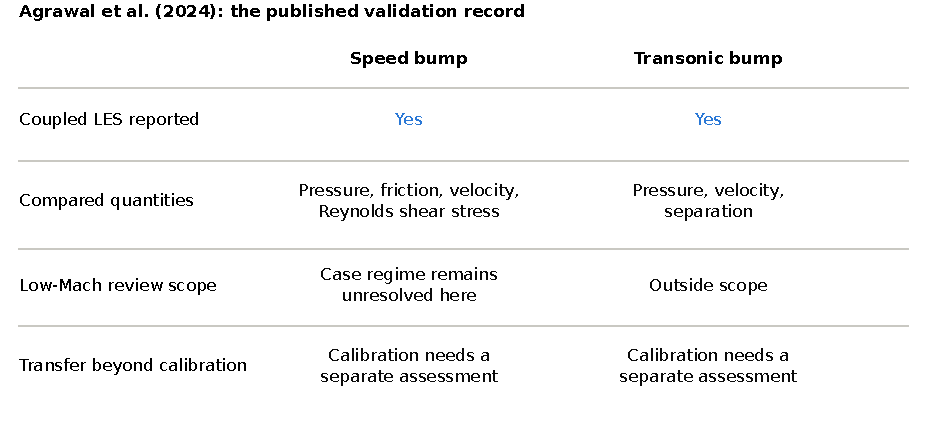
\includegraphics[width=\textwidth]{../figures/fig2_record.pdf}
\caption{Eight comparisons with different diagnostic quantities~\cite{Hayat2024preprint,BaeKoumoutsakos2022,LozanoDuranBae2023,Mukha2025,ZhouBae2024,Agrawal2024,Dupuy2023graph,Jones2015}. \textbf{a}, Refinement brings the velocity sample into the training interval. Circles and diamonds reproduce the two stress-error columns in Mukha et al., Table VII. \textbf{b}, Signs give mean chordwise friction at $x/Y=0$, inside the bubble. A value within the line width of zero is marked $\sim$0. The asterisk identifies the preprint used for these signs. \textbf{c}, The upper pair measures mean velocity in the first cell under prescribed mean traction. The lower pair measures predicted mean skin friction. \textbf{d}, The downstream zero of mean shear locates step reattachment against a wall-resolved benchmark. $N$ counts graph message-passing steps. The diffuser runs change transverse mesh and wall treatment together.}\label{fig:record}
\end{figure*}

\subsection{Stress direction and momentum balance}
In the unswept bubble of Hayat and Park~\cite{Hayat2024preprint,HayatPark2025}, the equilibrium calculation gives reversed mean velocity near the wall. Its mean chordwise skin friction approaches zero, with no negative interval distinguishable at the plotted line width. The matching point lies above this thin reversed layer. A monotone profile fitted to forward \emph{mean} velocity there misses the reversal, while a model solving non-equilibrium partial differential equations gives clearly negative mean friction. With $35^\circ$ sweep the reversed layer reaches the matching point and all three models give negative mean chordwise friction (Fig.~\ref{fig:record}b). The instantaneous alignment test requires the paired samples of Fig.~\ref{fig:loop}b.

Hayat and Park also found compensating errors in the swept case using Renard and Deck's decomposition of chordwise friction from the mean kinetic-energy budget~\cite{RenardDeck2016}. Pressure and convection in the momentum integral of Eq.~\eqref{eq:balance} require their own test for compensation~\cite{Larsson2016}. On the NASA wall-mounted hump, Park~\cite{Park2017} found comparable results for equilibrium and non-equilibrium models upstream, with better non-equilibrium predictions in separation and recovery. Local friction distinguishes regions that an integral over the whole hump could obscure.

At $Re_\tau=50{,}000$, Bae and Koumoutsakos~\cite{BaeKoumoutsakos2022} reduced the wall-normal grid spacing from $0.05\delta$ to $0.01\delta$ while keeping the wall-parallel spacings fixed. The sampling height moved from 5,000 to 1,000 wall units, inside the training interval $150<h^+<1200$. For the velocity-based policy, the signed error in predicted friction velocity changed from about $-29$ to $+3\,\%$. Refinement changed the LES input as well as its height. The policy using log-law variables retained small errors over the tested range, so a training-height limit depends on the input representation.

The direction of the applied pressure gradient provides a further test. Lozano-Dur\'an et al.~\cite{LozanoDuran2019} imposed a sudden spanwise pressure gradient in a channel at $Re_\tau\simeq1000$. One outer time unit later, the spanwise wall-stress error was about $10\,\%$ for the equilibrium model and $2\,\%$ for each of two non-equilibrium models. Yet all three missed the initial fall in streamwise wall stress. In the three-dimensional boundary layer of a bent square duct, Hu et al.~\cite{Hu2023} found the wall-stress direction of a non-equilibrium model closer to experiment than that of an equilibrium model, the two differing by up to about $5^\circ$ within the bend. Stress magnitudes were comparable and mean velocity profiles almost identical. The authors conclude that the LES away from the wall did not feel the difference in direction. After a sudden adverse pressure gradient in a half-channel, Hansen et al.~\cite{Hansen2023} added a second mode to the law of the wall. At one instant of the stronger case the equilibrium model gave $0.67$ and the augmented model $0.40$ of the initial wall stress against $0.31$ in DNS, errors of $116$ and $29\,\%$. At a gradient ten times weaker the augmented model was slightly less accurate.

\begin{table*}[t]
\caption{Examples that discriminate parts of a wall-modelled calculation. A reported mechanism is distinguished from what the comparison directly establishes. The source version is identified in the text and bibliography; the accompanying support register gives locations. These examples are not a frequency sample or an exhaustive taxonomy.}\label{tab:evidence}
\footnotesize
\begin{tabular*}{\textwidth}{@{\extracolsep{\fill}}>{\raggedright\arraybackslash}p{0.15\textwidth}>{\raggedright\arraybackslash}p{0.37\textwidth}>{\raggedright\arraybackslash}p{0.41\textwidth}@{}}
\toprule
Question & Evidence and inference & Qualification or useful next test \\
\midrule
States returned & A stress constrained to align with forward velocity at $h$ cannot represent negative shear below it. The thin-bubble comparison illustrates this limit~\cite{Hayat2024preprint}. & The analytic restriction is decisive for that state; a coupled comparison of different model formulations also changes retained physics. Test sign and direction separately from stress magnitude. \\
Retained balance & A term decomposition reveals cancellation between erroneous contributions despite reasonable final friction~\cite{Hayat2024preprint}. & A correct total does not verify its components. Compare signed budgets and, where possible, a controlled term ablation; allow for the breakdown of the thin-layer approximation. \\
Input information & The building-block study separates internal error using exact-for-mean outer modelling from total error with practical closures~\cite{LozanoDuranBae2023}. & Those calculations intentionally change the input-generating system. Prescribed inputs can diagnose the map but cannot establish coupled accuracy. \\
Coupling & Fixed-$h$ refinement tests input resolution~\cite{Larsson2016}; a spectral-element manuscript distinguishes imposed traction from the wall gradient~\cite{Mukha2024preprint}. & State the discretisation and traction implementation. Refinement can also alter a model's input stencil; it need not isolate one mechanism. \\
Outside the model & A bump calculation retains reference mean stress and varies the outer closure, with different separation predictions~\cite{Zhou2024preprint}. & Correct mean traction does not make instantaneous traction, numerics or the outer flow exact. The result identifies sensitivity in that configuration. \\
\botrule
\end{tabular*}
\end{table*}


\subsection{Sampling, feedback and the outer flow}
Lozano-Dur\'an and Bae~\cite{LozanoDuranBae2023} separated two sources of error in a zero-pressure-gradient boundary layer. Their exact-for-the-mean subgrid-scale closure supplies an outer mean velocity close to the reference. Downstream of the inlet adjustment they report internal wall-stress errors below $0.5\,\%$ for the building-block wall model and about $2\,\%$ for the equilibrium wall law. With practical outer closures the reported total errors are generally $5$--$15\,\%$. Locally, the equilibrium wall law with the dynamic Smagorinsky closure reaches about $19\,\%$ at $Re_x=10^6$ (Fig.~\ref{fig:contrast}b). In their separating Poiseuille--Couette flow the building-block model is closer to the DNS wall stress with dynamic Smagorinsky at both pressure gradients that resolve an order. With the Vreman closure the equilibrium law is closer at four of seven (their Fig.~11d).

Against NASA Juncture Flow measurements, the building-block model improved the velocity profile relative to the equilibrium law. Appreciable error persisted in the separated wing--fuselage corner, where the authors report one grid point across the bubble. On the high-lift Common Research Model at $7^\circ$, keeping the dynamic Smagorinsky closure and mesh fixed, replacing equilibrium with their building-block wall improves the pitching moment while taking the lift farther from the experiment (their Fig.~15a,c). In the fourth AIAA High-Lift Prediction Workshop nine participants computed this configuration with wall-modelled LES or lattice-Boltzmann methods~\cite{Kiris2023}. All but two submissions gave a maximum lift coefficient that the summary calls fairly accurate, most between $2.48$ and $2.57$. Pitching moments scattered more at $7^\circ$ and $21.4^\circ$, and at least 250 million cells were needed for the outboard loading.

In a channel, coupling can displace the logarithmic mean velocity profile. Kawai and Larsson~\cite{KawaiLarsson2012} traced a source of error to numerical and subgrid-scale errors in the first few off-wall cells. Sampling farther from the wall and refining the grid at fixed physical $h$ probe different effects~\cite{Larsson2016}. Yang et al.~\cite{YangParkMoin2017} found that filtering the velocity used by the wall model could alleviate the mismatch in their calculations. Rezaeiravesh et al.~\cite{Rezaeiravesh2019} repeated eight channel calculations at nominal $Re_\tau=5200$ with and without Spalding's law, holding the grid and each combination of convection scheme and subgrid closure fixed (Table~\ref{tab:decisions}). Adding the wall law reduced the absolute friction-velocity error in all eight. The maximum outer mean-velocity discrepancy over $0.2\le y/\delta\le1$ increased for all four linear-differencing cases, by $0.10$ to $3.65$ percentage points, and decreased for all four cases using the blended LUST scheme.

In the fixed-bulk-flow channel of Mukha, Bensow and Liefvendahl~\cite{MukhaBensow2021}, the friction Reynolds number is an output. With Spalding's law sampled at the second off-wall cell, halving the hexahedral grid spacing from $\delta/15$ to $\delta/30$ moved the sample towards the wall. The signed friction Reynolds number error went from $+0.24\,\%$ to $-1.66\,\%$. This tests grid and sampling together. Mart\'inez-S\'anchez and Lozano-Dur\'an~\cite{MartinezSanchez2026} forecast future wall shear from prescribed velocity planes of channel DNS, a response to supplied inputs that leaves solver feedback untested.

Mukha, Parsani and Schlatter~\cite{Mukha2025} applied the same nonlinear law \emph{a priori} to the mean velocity from each spectral-element channel run. The absolute mean-stress error decreased on meshes M1 and M2 and increased on M3 (Fig.~\ref{fig:record}a). The coupled values in their Table VII differ from those in Table III, which the caption calls repetitions, and either gives the same three directions.

Zhou and Bae~\cite{ZhouBae2024} prescribed DNS mean traction on a Gaussian bump. On the baseline grid the mean streamwise velocity at $x_2/L=2.38\times10^{-4}$ reversed with Vreman coefficient 0.025 and stayed forward with 0.07 (their Fig.~7). Holding the latter coefficient fixed and changing the effective-viscosity wall condition from equilibrium to non-equilibrium produced a friction-defined bubble about $0.14L$ long while the first-cell mean velocity still showed essentially no reversal (their Figs.~14--15). The first isolates sensitivity to the outer closure. The second shows that velocity and friction locate different boundaries of a thin reversed layer.

Some methods resolve small near-wall regions and couple them to a coarser outer LES. In channel flow at $Re_\tau=4200$, Sandham et al.~\cite{Sandham2017} kept the near-wall grids fixed and refined the outer grid. The centreline mean velocity went from $3\,\%$ below DNS to less than $1\,\%$ below it, while the root-mean-square streamwise fluctuation moved farther from DNS above about 25 wall units. Grid stretching and the LES time step also changed. Chen and He~\cite{Chen2023} varied the exchange between embedded fine-grid blocks and a coarse grid in a tripped boundary layer. At the outlet ($Re_\theta\simeq1000$), we read $U^+\simeq19.3$ with the source terms suppressed and $16.6$ with them included, against $16.4$ in DNS at $y^+=100$ (their Fig.~25). The remaining difference is smaller than the width of the reference curve.

On the 2024 AIAA smooth ramp, four participating groups compared the streamwise zeros of mean skin friction with a common DNS. Three groups approached the DNS crossings on their finest meshes, yet only two showed apparent convergence and some sequences were non-monotone~\cite{Garmann2024}. Agreement on the upstream velocity profile at $x/L=-0.62$ did not determine the downstream reattachment location.

\begin{figure*}[t]
\centering
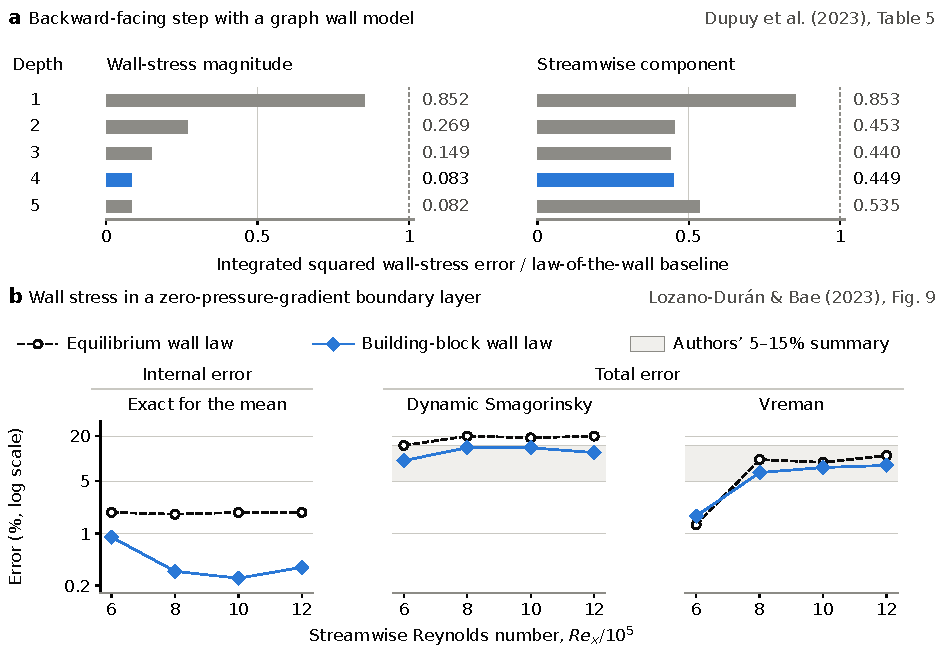
\includegraphics[width=\textwidth]{../figures/fig3_contrast.pdf}
\caption{Two comparisons of coupled wall-stress predictions. \textbf{a}, Dupuy et al.~\cite{Dupuy2023graph}, Table~5, integrate squared stress errors over 14 step heights downstream. Each bar gives the ratio to its law-of-the-wall baseline. \textbf{b}, Local errors are read from Fig.~9(c,d) of Lozano-Dur\'an and Bae~\cite{LozanoDuranBae2023} at the four velocity-profile stations in their Fig.~9(a). Lines join these values on a common logarithmic scale. The exact-for-mean closure measures internal error. Shading marks the authors' $5$--$15\,\%$ summary for practical closures. At $Re_x=10^6$ the equilibrium/dynamic Smagorinsky trace gives about $19\,\%$. Moving the digitised point across half a marker spacing and the stroke width gives roughly $18$--$21\,\%$.}\label{fig:contrast}
\end{figure*}

\subsection{Calibration, validation and transfer}\label{sec:scope}
A learned wall law receives the velocity available in its solver~\cite{Duraisamy2021,HuYang2026}. In an Ahmed-body study, Kamac{\i} and Kaya~\cite{KamaciKaya2021} used the measured drag to choose the combination of turbulence model and wall function, so agreement on that drag characterises the calibration. In periodic-hill LES at $Re_h=10{,}595$, Cato et al.~\cite{Cato2026} selected one algebraic model on mean friction and a second on mean velocity at 12 stations. The profiles highlighted at $x/h=2,3,6$ belong to the second objective, so their agreement demonstrates a fit. On a curved backward-facing step at $Re_h=13{,}700$, the friction-trained model captured much of the separated-region stress but overpredicted friction upstream and downstream of the bubble.

Zhang et al.~\cite{Zhang2026} applied a wall model trained in differentiable periodic-hill LES to a Gaussian bump ($Re_L=2\times10^6$) and a smooth ramp ($Re_L=6.67\times10^5$). At the bump's upstream station all three formulations gave similar mean velocity. Farther downstream their third learned formulation recovered separated velocity profiles missed by the pressure-gradient and simpler learned variants. On the ramp the reference DNS also helped generate the inlet turbulence.

To assess transfer, record which data determined the coefficients, thresholds and model structure. Raje and Duraisamy~\cite{Raje2025} selected the limiter coefficient of their dynamic-slip formulation through numerical experiments across Reynolds numbers and configurations. A coupled test on one of those flows lies within the selection range. A withheld realisation there and an extrapolation to a new range answer different questions. In our collection, 33 reports test a fitted treatment at 110 conditions outside the data reported as used to fit it. Nine tests in four reports state that the target was withheld from training and model selection or apply unchanged coefficients published earlier by other authors. Six of the nine come from one study~\cite{LozanoDuranBae2023}, and one, a rough-wall channel, lies outside our primary scope. Only one of the nine lies within the stated ranges of the fitting set in a flow of that set. Four exceed a stated range, three are other flows and one source does not describe its fitting set. Sixty compare variants of the treatment at the target or select with it, and 41 remain unresolved. Excluding borderline reports the counts are 102 conditions in 29 reports (9, 55 and 38); within the primary scope, 100 in 30 (8, 53 and 39).

In Agrawal et al.'s NASA/Boeing speed-bump test at $Re_L=2\times10^6$, the sensor-based wall model predicts negative mean skin friction on the medium grid while the equilibrium model stays attached~\cite{Agrawal2024}. On the fine mesh both separate. Downstream velocity and Reynolds shear stress improve on the coarse and medium grids, with residual differences from the quasi-DNS.

\noindent For a fixed solver, ranking can depend on the observable even at a single station. Take Zhou and Bae's learned-wall-model bump calculations~\cite{DiZhou2024} on the fine mesh with dynamic Smagorinsky closure at $Re_L=2\times10^6$ and $x/L=-0.4$ (Table~\ref{tab:decisions}). The learned wall gives closer friction against a value interpolated between two measured stations. Over $0.002\lesssim y/L\lesssim0.060$ the equilibrium wall gives the smaller mean absolute velocity discrepancy, and the authors also find its velocity better here. The difference arises below $y/L\approx0.016$, in about the first 16 cells, where the learned profile exceeds the measurements by about 0.05. Above $y/L=0.02$ both lie above the measurements, by about 0.011 and 0.007, an order that would reverse if the measured profile were 0.009 higher. In the pressure recovery ($0.20<x/L<0.39$) both walls miss the ten measured values of $C_p$, on average by 0.20 and 0.24, and the learned wall is farther at each, a difference the authors call minor. The same runs can support a friction prediction at this station and a velocity prediction only over a specified height range.

The separation and reattachment points of a periodic hill test two parts of the same mean friction curve. Five retrieved studies tabulate both crossings for the standard hill at $Re_H=10{,}595$, with a reference for both and a change of wall treatment on the same nominal mesh~\cite{Krank2016,Krank2018,ZhouFEL2025,DiZhou2024,Boxho2025}. Of nine such comparisons, five move both crossings closer, by $0.06H$ to about $2H$. Two move them in opposite directions, and neither source reports a sampling uncertainty for a crossing. On Zhou et al.'s finest unit-slope mesh~\cite{ZhouFEL2025}, separation moves from $0.31H$ to $0.29H$ against $0.22H$ and reattachment from $4.26H$ to $4.18H$ against $4.35H$. Boxho et al.~\cite{Boxho2025} move separation $0.035H$ farther and reattachment $0.28H$ closer. Krank and Wall~\cite{Krank2016} print the separation point without the wall model as $0.2$, which leaves its $0.05H$ change unresolved, and their reattachment gain against the resolved LES is a loss against the experiment in the same table. Zhou and Bae and Boxho et al. test on the hill used for training, and Zhou et al.'s unit slope lies between their two training slopes. These tables do not establish a trade-off between the two crossings.

\subsection{Improvement over a baseline and accuracy against a reference}\label{sec:comparison}
In coarse-grid RANS of a backward-facing step, Fogliatto and Clifford~\cite{Fogliatto2024} found that replacing a standard wall function with a wake function brought the spatially averaged friction coefficient closer to the reference, while the streamwise velocity profiles changed little at a given resolution. On a Gaussian bump at Mach 0.17, Arranz et al.~\cite{Arranz2024} found that their building-block model improved pressure and skin friction downstream of the crest ($x/L>0.1$) relative to equilibrium-wall-law calculations. Upstream friction remained inaccurate. Retaining the learned wall-stress model and replacing its learned subgrid stresses with a dynamic Smagorinsky closure lost much of the separation improvement (their Fig.~11b), an outer-closure contribution on that grid.

Dupuy et al.~\cite{Dupuy2023graph} report two spatial integrals of squared wall-stress error behind a backward-facing step. With four message-passing steps the graph model gives $0.067$ for stress magnitude and $0.308$ for the streamwise component, against $0.806$ and $0.686$ for the law of the wall. The source labels both columns $\mathrm{N}^2/\mathrm{m}^2$. Each error falls, to about $8\,\%$ and $45\,\%$ of its baseline (Fig.~\ref{fig:contrast}a). A fifth step gives $0.066$ and $0.367$, a magnitude gain of one unit in the last printed place that remains unresolved. In the same study the downstream zero of mean streamwise wall shear lies at $x_r/h_s\approx4.7$ for the log law, $5.2$ for the four-step graph model and $6.0$ for the wall-resolved reference, where $h_s$ is the step height (Fig.~\ref{fig:record}d). To the precision of the plotted traces, the shortfall falls from about $1.3$ to $0.8$ step heights. The two integrals in Fig.~\ref{fig:contrast}a weight errors over the whole downstream interval and do not give the size of this shift.

Two complete calculations can be compared even when their meshes differ. In the diffuser of Jones and Utyuzhnikov~\cite{Jones2015}, the interface method recovered inclined-wall recirculation missed by the log law and slightly improved the total pressure drop. Both missed the pressure curvature near the outlet. The transverse grids differed, leaving the effect of the wall treatment unresolved. Within the interface method, replacing the Robin condition on turbulent kinetic energy with a Dirichlet condition removed the bubble with the linear viscosity profile and shortened it with the Duprat profile (their Fig.~7b).

He et al.~\cite{HeRVACS2026} compared unsteady standard $k$--$\varepsilon$ wall treatments in a baffled natural-convection passage, outside our primary scope, on one mesh of 11,683 cells. From their data deposit~\cite{HeRVACSData} we integrated the squared difference between each mean wall profile and the DNS reference over the common wall length. On the right baffle face, switching from the scalable to the two-scale treatment reduces the root-mean-square shear discrepancy from $2.44$ to $0.85$~mPa and increases the heat-flux discrepancy from $118$ to $155$~W\,m$^{-2}$. On the other three walls both decrease. With the SST closure and its all-$y^+$ baseline, the switch increases both on the hot wall.

\begin{figure*}[t]
\centering
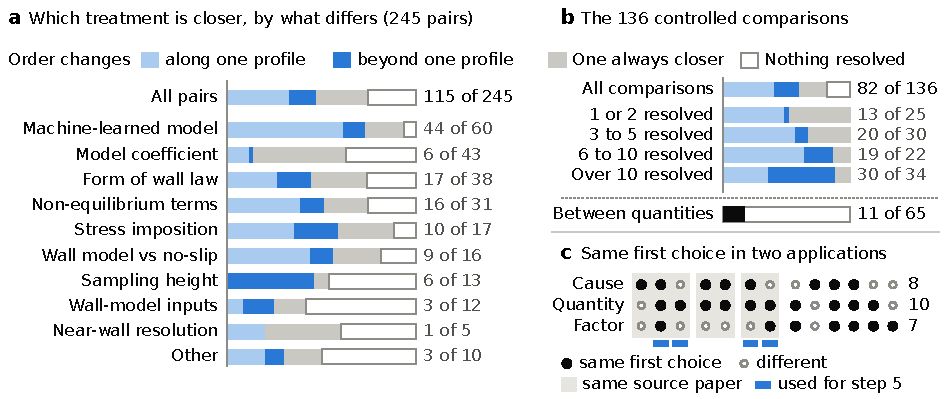
\includegraphics[width=\textwidth]{../figures/fig4_outcomes.pdf}
\caption{Which of two wall treatments lies closer to the reference. \textbf{a}, Pairs of treatments in the 136 controlled comparisons, by what distinguishes them. Light blue pairs change order only along one profile. Blue pairs change it between conditions or quantities. In grey pairs one treatment is closer wherever a direction is resolved. \textbf{b}, The same for the comparisons, together and by the number of individual comparisons each resolves. The black bar is counted over the 65 comparisons that resolve two classes of quantity under one condition. Excluding borderline reports the first bar is 79, 27 and 24 of 130. Within the primary scope it is 74, 26 and 16 of 116. \textbf{c}, First choices of two applications of the five questions to 13 retrospective cases. Grey bands mark cases that share a source paper. Four cases were used to write step 5.}\label{fig:outcomes}
\end{figure*}

\subsection{Which treatment is closer}\label{sec:order}
For each of the 136 controlled comparisons in the 58 reports we recorded every quantity that the source compares with a reference for both treatments, 981 rows in all with 55 thermal rows kept apart, and which treatment lies closer (Sec.~\ref{sec:methods}). A direction is resolved only if it holds to the printed digits or exceeds the stroke width of the plotted curves, a test that $48\,\%$ of 2,250 individual comparisons fail.

In 29 comparisons one treatment is closer wherever a direction is resolved, and only six of these resolve every row. In 25 nothing is resolved. In 82 the order changes (Fig.~\ref{fig:outcomes}b), a number that unresolved rows could raise to at most 130. In 55 of the 82 the only change lies along a single profile, where each treatment is closer over part of the range. In the other 27 it changes beyond one profile. In 25 the order changes between conditions. A single factor separates opposite orders for the grid in nine comparisons, the Reynolds number in six, and the convection scheme and the outer closure in four each (factors coded once). In 11 of the 65 comparisons that resolve two classes of quantity under one condition the order differs between them, for mean velocity and wall stress in 6 of 19. A change of order appears in 44 of the 58 reports, and in 32 of 40 groups when reports sharing a treatment, computation or benchmark are joined.

These counts depend on how much a source reports. Of the 25 comparisons that resolve one or two individual comparisons, the order changes in 13, in one of them beyond a single profile. Of the 34 that resolve more than ten it changes in 30, in 18 beyond a profile, and four keep one order. Of the 29 comparisons with one order, 22 resolve five or fewer. A treatment that is closer throughout is documented mainly where little is compared.

Changes beyond one profile are not confined to complex flows. Fifteen of the 27 occur in developed channels, pipes or flat-plate boundary layers (64 comparisons) and 11 in flows with separation, streamwise pressure gradient, three-dimensionality, roughness or rotation (64), by a keyword rule applied once to the recorded case. In the developed flows the separating factor is the grid or the Reynolds number in five comparisons each and the convection scheme in three. In the pulsating channel of Fowler et al.~\cite{Fowler2023} the order changes with frequency and with quantity. Their multi-time-scale model holds the wall-stress amplitude at the Stokes value at the two highest forcing frequencies, where the equilibrium law gives about a quarter and a sixth of it. At intermediate frequencies the equilibrium law has the closer amplitude of the periodic Reynolds shear stress.

Grouped by what distinguishes the two treatments (Fig.~\ref{fig:outcomes}a), a changed coefficient most often leaves one order, in 21 of 43 pairs. Such a pair resolves $1.5$ individual comparisons on average, against $5.5$ for a pair with a machine-learned model. A machine-learned model changes the order in 44 of 60 pairs from 11 reports, in 37 of them only along one profile. Where separation or reattachment points are compared with a designated baseline, the alternative is closer in 18 of 24 pairs and the baseline in none. For wall stress the split is 26 to 15, with 37 changing and 10 unresolved. Of the 18 pairs in which one treatment has the closer crossing and wall stress is also compared, the wall-stress order changes along the wall in 16. A closer zero of the friction curve does not make the curve closer. In 117 of the 172 pairs with a designated baseline the alternative is the authors' own proposal, so these splits carry the selection of what is published. The counts describe the retrieved collection, not a frequency for the literature.

\section{From a published result to a planned use}\label{sec:procedure}
Experimental validation estimates accuracy for a specified quantity and conditions, accounting for experimental, input and numerical uncertainties~\cite{OberkampfTrucano2002,ASMEVV20}. The application supplies the tolerance~\cite{Eca2022}. Table~\ref{tab:checklist} adds questions specific to a wall-modelled calculation. Table~\ref{tab:decisions} works three published comparisons through them.

\begin{table*}[t]
\caption{Checklist for a named model and a planned flow, quantity, tolerance and numerical set-up. A missing fact gives \emph{unknown}, not evidence of failure or success. The checklist is a proposal for structuring judgement; its predictive value has not been established.}\label{tab:checklist}
\footnotesize
\begin{tabular*}{\textwidth}{@{\extracolsep{\fill}}p{0.11\textwidth}p{0.31\textwidth}p{0.51\textwidth}@{}}
\toprule
Step & Question & Evidence to record and consequence \\
\midrule
1. Quantity & What is to be predicted, and does the set-up constrain it? & Specify quantity, position, averaging, error measure and tolerance. Derive the relevant conservation constraint. Use a free quantity to assess constitutive accuracy; keep constrained quantities as balance checks. \\
2. Model & Which limitations could matter here? & Record output restrictions, retained terms, available inputs, calibration and tuning, and coupling. Identify relevant flow features and uncertainty. These are candidate explanations, not diagnosed causes. \\
3. Test design & What does the published test actually test? & Distinguish exact-input evaluation from coupled validation. Within coupled tests, distinguish calibration cases from documented transfer cases; unknown calibration remains unknown. Both in-range and out-of-range failures are informative. \\
4. Comparison & What improved, and is the result accurate enough? & Record the matched baseline and reference separately. Compare the same flow, grid, closure, height and spatial support. Keep relative benefit, absolute error, tolerance and uncertainty as separate assessments. No matched baseline means benefit is unassessed; it does not invalidate a reference comparison. \\
5. Planned use & How far can the evidence be extended? & List differences in model version, flow, parameters, quantity and numerics. A direct match supports the stated result within its uncertainty. An extension needs a physical argument and relevant sensitivity evidence at the required tolerance. Otherwise withhold assurance and propose a comparison; do not infer failure. \\
\midrule
Next test & \multicolumn{2}{p{0.85\textwidth}}{Name the uncertainty the test addresses. Specify model and baseline, flow, forcing, grid, closure, matching height, quantities, reference and uncertainty estimates. Score the intended quantity alongside other affected outputs. Use an ablation or controlled change to test a candidate mechanism, recording what still changes with it. State what the test can establish and what remains unresolved. If no reference is available, sensitivity or cross-model agreement alone cannot establish absolute accuracy.} \\
\botrule
\end{tabular*}
\end{table*}


Write the signed discrepancies for model and baseline as $d_m=q_m-r$ and $d_b=q_b-r$, using the same reference $r$. It cancels from $d_m-d_b=q_m-q_b$. It can still reverse the ranking by absolute error if it crosses the midpoint of the predictions. To resolve improvement, propagate the joint uncertainty of $(q_m,q_b,r)$ through $|d_b|-|d_m|$ and check that its lower bound exceeds zero. Use each shared reference or input once per realisation, retaining correlated discretisation and sampling errors. A variance calculation for the signed change includes $-2\,\mathrm{Cov}(d_m,d_b)$.

For agreement within a tolerance $T$, form an interval for the signed discrepancy, using deterministic error bounds or an interval with stated coverage and assumptions. Containment in $[-T,T]$ supports agreement at that scope and coverage. For a symmetric half-width $u$ this requires $|d_m|+u\le T$. A disjoint interval supports a miss. Partial overlap leaves the decision open. A standard deviation or digitisation precision alone supplies no such interval.

\begin{table*}[t]
\caption{Three published comparisons worked through to a next test. Tolerances are illustrative. Intervals reflect digitisation or printing precision alone. None of the three sources gives a joint interval for sampling, discretisation and reference uncertainty.}\label{tab:decisions}
\footnotesize
\begin{tabular*}{\textwidth}{@{\extracolsep{\fill}}>{\raggedright\arraybackslash}p{0.092\textwidth}>{\raggedright\arraybackslash}p{0.18\textwidth}>{\raggedright\arraybackslash}p{0.21\textwidth}>{\raggedright\arraybackslash}p{0.435\textwidth}@{}}
\toprule
 & Step reattachment~\cite{Dupuy2023graph} & Fixed-flow channel~\cite{Rezaeiravesh2019} & Bump station $x/L=-0.4$~\cite{DiZhou2024} \\
\midrule
Prediction, tolerance and reference & Mean reattachment within $0.5h_s$ of the wall-resolved LES of the same study & Friction velocity within $2\,\%$ and outer mean velocity within $1\,\%$ of channel DNS & Skin friction within $10\,\%$ and mean velocity within $0.01U_\infty$ of oil-film and particle-image measurements \\
Published comparison & Log law $4.7$, graph model $5.2$, reference $6.0$, read to $0.1$. Discrepancies $-1.3$ and $-0.8h_s$ & With Spalding's law the friction error falls in 8 of 8 pairs. The outer error falls in 4 of 4 with LUST, to $0.58$--$0.76\,\%$, and rises in 4 of 4 with linear differencing, to $1.01$--$6.03\,\%$ & Fine mesh: $10^3C_f$ of $3.09$ and $2.18$ against $2.35$, read to $0.1$: $+31$ and $-7\,\%$. Velocity discrepancy $0.010$ and $0.016U_\infty$ for the equilibrium and learned walls. Coarse and medium meshes: friction $+54$ and $-5\,\%$, $+42$ and $+2\,\%$. Velocity on the 117 heights common to the three meshes: $0.013$ and $0.012$ (coarse), $0.012$ and $0.012$ (medium), $0.010$ and $0.014$ (fine) \\
Uncertainty reported & None for a crossing & Printing to $0.01\,\%$ only & Friction bias within $2\,\%$ and freestream speed $0.4\,\%$~\cite{Gray2023}. Random error only for the velocity field. Statistics span 1.5 flow-through times \\
Attribution & A shift of $0.5h_s$ follows the change of wall treatment in the coupled calculation. The remaining $0.8h_s$ is unattributed & Each change follows the wall law under one scheme and closure. The scheme sets the sign for the outer velocity & The changes follow the complete wall treatment. The equilibrium wall samples the second off-wall cell, which moves with the mesh. Below $y/L=0.02$ its discrepancy falls with refinement from $0.023$ to $0.014$ and $0.008$. The learned wall's stays between $0.025$ and $0.032$ \\
Ordinary validation & The point estimate misses the tolerance. Without a grid-convergence estimate no validation conclusion follows & Both errors lie within tolerance with LUST on the printed values. The outer error exceeds it in 4 of 4 with linear differencing & Equilibrium friction misses the tolerance on every mesh. Learned friction meets it on the coarse and medium meshes and is open on the fine mesh, at $-11$ to $-3\,\%$ within digitisation precision. The equilibrium velocity discrepancy lies on the tolerance and is undecided. The learned one exceeds it. The velocity order over all heights is resolved only on the fine mesh \\
Next test & Refine with the sampling height and graph points fixed in physical space. Vary the height on one mesh & Repeat the pair with the intended scheme. Under a prescribed pressure gradient, assess bulk velocity and profile & Refine at a fixed physical sampling height. Name the quantity and height range: on every mesh the equilibrium wall is closer below $y/L=0.02$ and the learned wall above it, $0.011$ against $0.007$ on the fine mesh \\
\botrule
\end{tabular*}
\end{table*}


Behind the step both point predictions lie upstream of the benchmark. While that ordering holds, a shift of their common reference cancels from the gain of about $0.5h_s$ but changes each discrepancy against the tolerance. The closer crossing would meet it only if the benchmark lay $0.3h_s$ farther upstream. In the channel the smallest of the four increases of the outer error under linear differencing, from $2.98$ to $3.08\,\%$, is resolved by the printed digits alone. At the bump station the stated friction bias, within $2\,\%$~\cite{Gray2023}, cannot reverse the friction ranking. The velocity margin of $0.007U_\infty$ is less than twice the $0.4\,\%$ quoted for the freestream speed, and the velocity field has no stated systematic uncertainty. Above $y/L=0.02$ the learned wall is closer by $0.004U_\infty$, which equals that $0.4\,\%$.

Ordinary validation practice already supplies the comparison, the tolerance judgement and the missing uncertainty in each column. The wall-specific questions change the next test. For an unknown numerical error the general remedy is systematic grid refinement, and without an estimate of grid-convergence error Oberkampf and Trucano draw no validation conclusion~\cite{OberkampfTrucano2002}. When the wall law reads the first off-wall cells, refinement also moves its sampling point~\cite{KawaiLarsson2012,Larsson2016} and, for a graph model, its input points. The trend then mixes discretisation error with a change of model input. Two published series show the effect. In the fixed-flow channel above, the friction error changes sign as the second-cell sample moves towards the wall~\cite{MukhaBensow2021}. At the bump station the equilibrium wall also samples the second cell, and the velocity order of the two walls over all heights is resolved only on the finest of three meshes~\cite{DiZhou2024}. Dupuy et al.~\cite{Dupuy2023graph} identify alignment with the first off-wall velocity as a possible source of the step offset. A discriminating test refines with the same trained model, inlet and outer closure, interpolating velocity to the same physical sampling height and graph points. The sampling height is then varied on one mesh. A shift in the downstream zero of mean shear beyond its sampling uncertainty, which must account for time correlation~\cite{Oliver2014}, would establish sensitivity under these controls. A practitioner versed in wall modelling may choose this test unaided. Steps 2 and 3 make the choice explicit and tie it to recorded inputs.

The five questions were tried retrospectively on 13 cases, each a later study linked to earlier papers on the same treatment or a successor. Two independent applications of the questions each proposed a test from the earlier papers and the intended flow, forcing and quantity. Their first choices agreed on cause in 8 cases, quantity class in 10, factor to vary in 7 and all three in 3 (Fig.~\ref{fig:outcomes}c). Both called for more evidence in every case, so the set contains no use with adequate evidence and cannot show whether the questions merely favour further testing. Four cases had informed the final step, shared source papers link the 13 into nine groups, and outcomes were known at selection. The exercise shows that the questions can be answered from published material and that they do not determine a unique test.

A test of benefit would be made before the reference outcome is known, on planned uses assembled from published tests, each with a quantity, a tolerance and the documentation available beforehand. The collection offers a seed. The one withheld test inside the stated training ranges of its model, a channel with a sudden spanwise pressure gradient~\cite{LozanoDuranBae2023}, is a candidate for adequate evidence. The step, the bump station and a channel pair with linear differencing in Table~\ref{tab:decisions} are uses with inadequate evidence. Practitioners assigned at random to ordinary validation documentation with or without the five questions would record the decision to proceed, a predicted error interval and the next test. Once the reference is revealed, a false acceptance is a decision to proceed that misses the tolerance, and an excess investigation is a further calculation requested although the tolerance was met. The comparison reports the loss $c_\mathrm{FA}n_\mathrm{FA}+c_\mathrm{EI}n_\mathrm{EI}$ over a range of cost ratios, with uses that share a model or benchmark forming one cluster. Detecting a fall in false acceptance from $30$ to $10\,\%$ with $80\,\%$ power needs about 60 independent decisions in each arm.

\section{Implications and limits}\label{sec:outlook}
To transfer a wall law between solvers, report the physical sampling height, local grid spacing and filter. A point sample and a time mean at the same height are different inputs. The applied traction and the stress inferred from the resolved gradient allow a check on the discrete wall force.

Extending these conclusions to rough walls, wall heat flux or high-Mach-number flow requires evidence for the effects of surface texture, heat transfer or compressibility on the intended prediction.

In the collection, the wall treatment that lies closer to the reference changes between conditions or quantities in 27 of 136 controlled comparisons and only along a single profile in 55 more. It changes more often the more a source compares, and one order survives in four of the 34 comparisons that resolve most. A claim that a wall model transfers should name the quantity, the position and the condition, including grid and numerical scheme, for which it was tested.

These counts describe reports that could be retrieved and compared. Of the 735 reports sought, 615 had no accessible copy. Of the 136 comparisons, 102 were extracted once. Directions are resolved to digitisation or printing precision, without sampling or reference uncertainty. No evidence yet shows that the five questions improve decisions. That requires the comparison with ordinary practice set out above, made before the reference outcome is known.

\section{Methods}\label{sec:methods}
\textbf{Search and screening.} Four title-and-abstract searches of OpenAlex~\cite{Priem2022} covered wall functions for the Reynolds-averaged Navier--Stokes (RANS) equations, LES wall conditions, inner--outer models and learned stress estimators, from 1 January 2000 to 16 November 2026. Box~1 reports each stage in the terms of PRISMA 2020~\cite{Page2021}, and the protocol gives each search as run.

\textbf{Eligibility.} An eligible report names a wall treatment or wall-stress estimator and contains an identifiable test that compares a quantity with a reference. The primary scope is turbulent flow of a single-phase Newtonian fluid with constant properties and no buoyancy over smooth walls at Mach numbers up to 0.3. Twelve eligible reports are borderline: five use near-wall methods on grids that reach the viscous sublayer, four test stress estimators never presented as wall models and three had disputed eligibility. Counts are given for the collection, excluding borderline reports and comparisons on grids that reach the sublayer, and within the primary scope.

\textbf{Data extraction.} Rules fixed before extraction name the facts that define the three groups of Box~1, and a script derives each group from the extracted facts. A second extraction, made from the rules and the sources alone, covered a random 30 of the 79 reports not used to write the rules and every candidate for the two rarer groups. A third, with both in view, reconciled each disagreement against the source.

\textbf{Which treatment is closer.} A printed value decides a direction only if it holds for every value that rounds to the printed digits and against every reference given. On a plotted curve one treatment is closer if the two differ by more than the stroke width over more than half of the range and no resolved stretch favours the other. The order changes along the profile if each treatment is closer over at least one resolved stretch, whatever its length. Directions are thus resolved to printing or digitisation precision, not to sampling or reference uncertainty. Rule, sample and agreement thresholds were fixed before extraction, which used the archived public copy of each report, an arXiv version for 37 of the 58. A second extraction covered a random 20 of the 58 reports. A third reconciled the six comparisons on which the two differed and changed the category of two.

\textbf{Synthesis.} Quantities and references differ between reports, so we count directions and pool no effect sizes, as in a synthesis without meta-analysis~\cite{Campbell2020}. The eight comparisons of Fig.~\ref{fig:record} are a purposive choice across four groups of geometries. The search did not uniquely determine them.

\backmatter
\bmhead{Data availability}
The accompanying data give the search protocol, the retrieved reports and their editions, every extraction with the reconciliation of each disagreement, source locations for Figs.~\ref{fig:record} and~\ref{fig:contrast}, the rows extracted for each controlled comparison with the 58 contributing reports, and the paired choices for the retrospective cases.
\bmhead{Code availability}
The accompanying scripts recompute the paired discrepancies, the three evidence groups, the closer treatment in each comparison and the agreement statistics, draw the figures and reproduce the wall-profile integrals from the public benchmark deposit.
\bmhead{Funding}
This work received no specific funding.
\bmhead{Author contributions}
To be decided when the author list is final.
\bmhead{Competing interests}
The authors declare no competing interests.
\bibliography{references}
\end{document}
